\chapter{Machine Learning Methodology} \label{Methods}
\ifpdf
    \graphicspath{{chapter_3/figures/PNG/}{chapter_3/figures/PDF/}{chapter_3/figures/}}
\else
    \graphicspath{{chapter_3/figures/EPS/}{chapter_3/figures/}}
\fi
\section{Introduction}
This section provides the details of materials and methods used in this project. As suggested by K. C. Chou in \cite{chou2011some}, we have followed the famous five steps: i) selection of a proper dataset; ii) representation of peptides using feature extraction; iii) selection of a classification algorithm; iv) evaluation methodology and v) establishment of a web server as a prediction tool. In the testing phase, we generate a large number of features based on the peptide sequences taken from the dataset. After that, the feature space is divided into thee parts and each are learnt using a weak classifier. The majority voting technique is used to provide with the final prediction decision from the weak classifiers. The ensemble is saved for the testing phase and used to predict anticancer property for any unknown peptide sequence. Rest of this section delineates the steps followed in this work.

\section{Benchmark Dataset}
In this project, we have used the training dataset constructed and presented by Wei et al. in \cite{wei2018acpred}. One major problem in the previous datasets prior to this work was the imbalance with the negative instances. This newly proposed dataset was based on previously available databases of ACPs \cite{tyagi2013silico,tyagi2014cancerppd,chen2016iacp}. Among all the available ACPs, CD-HIT \cite{li2006cd} was used to remove instances with 90\% or more similarity. From that 250 positive and 250 negative samples were selected to construct the training dataset. Table~\ref{tab:dataset} provides a summary pdf the dataset. Formally, the dataset $\mathbb{S}$ can be shown as below: 
$$\mathbb{S}=\mathbb{S}^+ \cup \mathbb{S}^-$$
Here, $\mathbb{S}^+$ and $\mathbb{S}^-$is the set of positive and negative instances respectively.
\begin{table}[h]
\centering
\begin{tabular}{c|c|c}
    \bf Type &\bf  Number of Instances &\bf Label  \\
    \hline 
    Anticancer Peptide & 250 & +1\\
    Non Anticancer Peptide & 250 & -1\\
    \hline
    Total & 500\\
\end{tabular}
\caption{Summary of the dataset. \label{tab:dataset}}
\end{table}


\section{Feature Collection}
After selection of the dataset, now we have to choose a proper way to represent each peptide $P\in \mathbb{S}$. Each peptide instance in the dataset is replaced by a set of features and thus converted into a feature vector formally shown as below:
$$P=[ f_1 f_2 f_3 \cdots f_n]$$

Note that, here each peptide sequences $P \in \mathbb{S}$ is a small string of amino-acids from the alphabet, $\Sigma$ that contains 20 different symbols. Here, $f_i$ is a feature extracted from the peptide instance. In this project, we generate different sequence based features that are easy to generate and also follows the common view that information flows from the genetic code and must be hidden in the peptide sequence itself. We provide a brief description of the features generated for our work

\begin{figure}[H]
\centering
 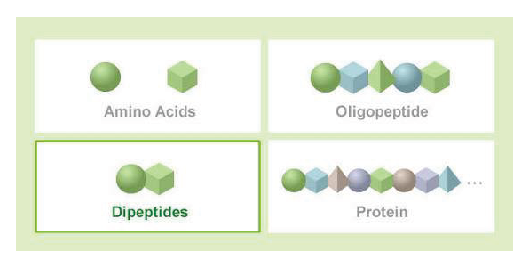
\includegraphics[width=0.5\textwidth]{f1.eps}
 \caption{Feature Collection}\cite{Anderson06}
\end{figure}

\subsection{Monomer Composition}
Monomer composition is simply the normalized frequency of the count of different amino acid monomers in the given peptide sequence. Since there are only 20 different amino acids, the number of features is 20. Here monomer composition is represented by $f_1$.

\begin{figure}[h]
\centering
 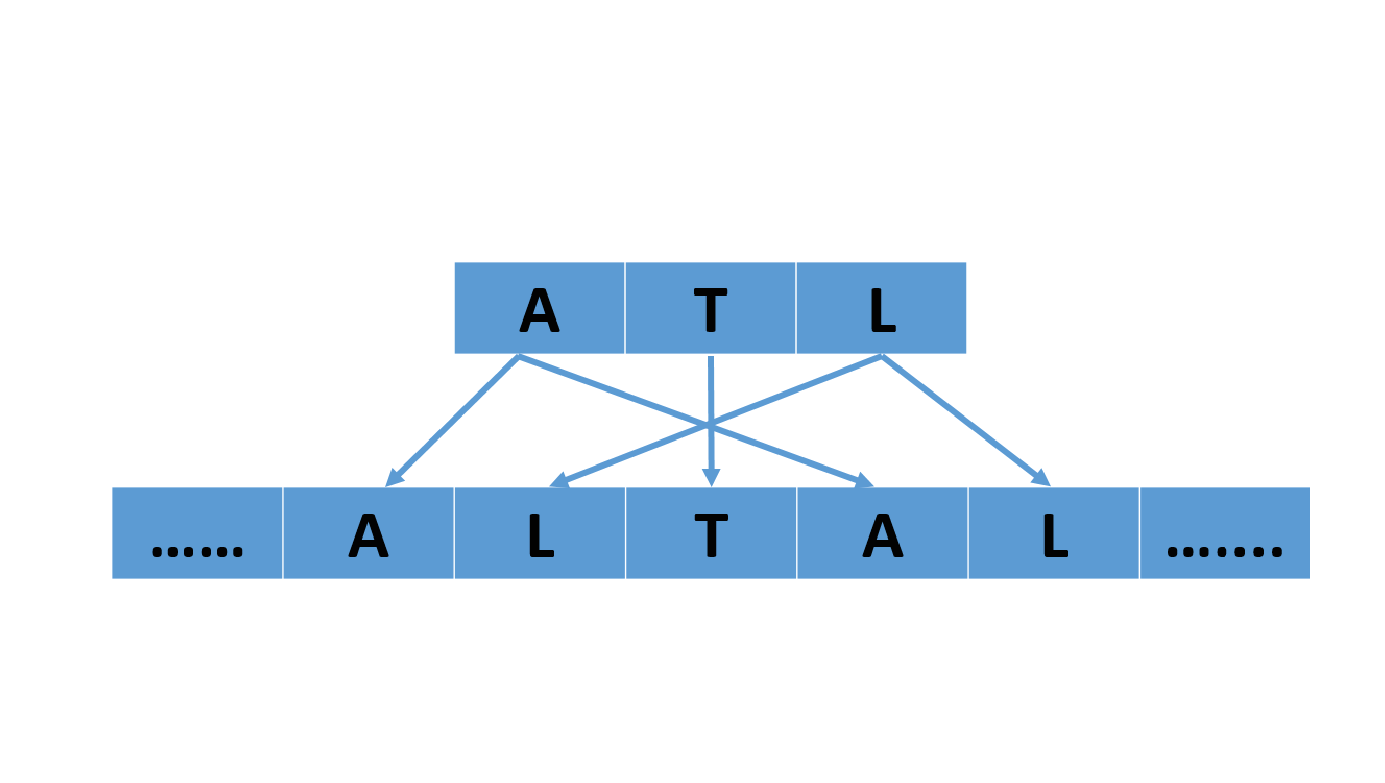
\includegraphics[width=0.7\textwidth]{mononew.eps}
 \caption{Monopeptide Composition}
\end{figure}

\subsection{Dipeptide Composition}
Dipeptide composition is the normalized frequency of the different dipeptides. Dipeptides are of 400 types and so is the number of features generated. Here monomer composition is represented by $f_2$.
    
\begin{figure}[H]
\centering
 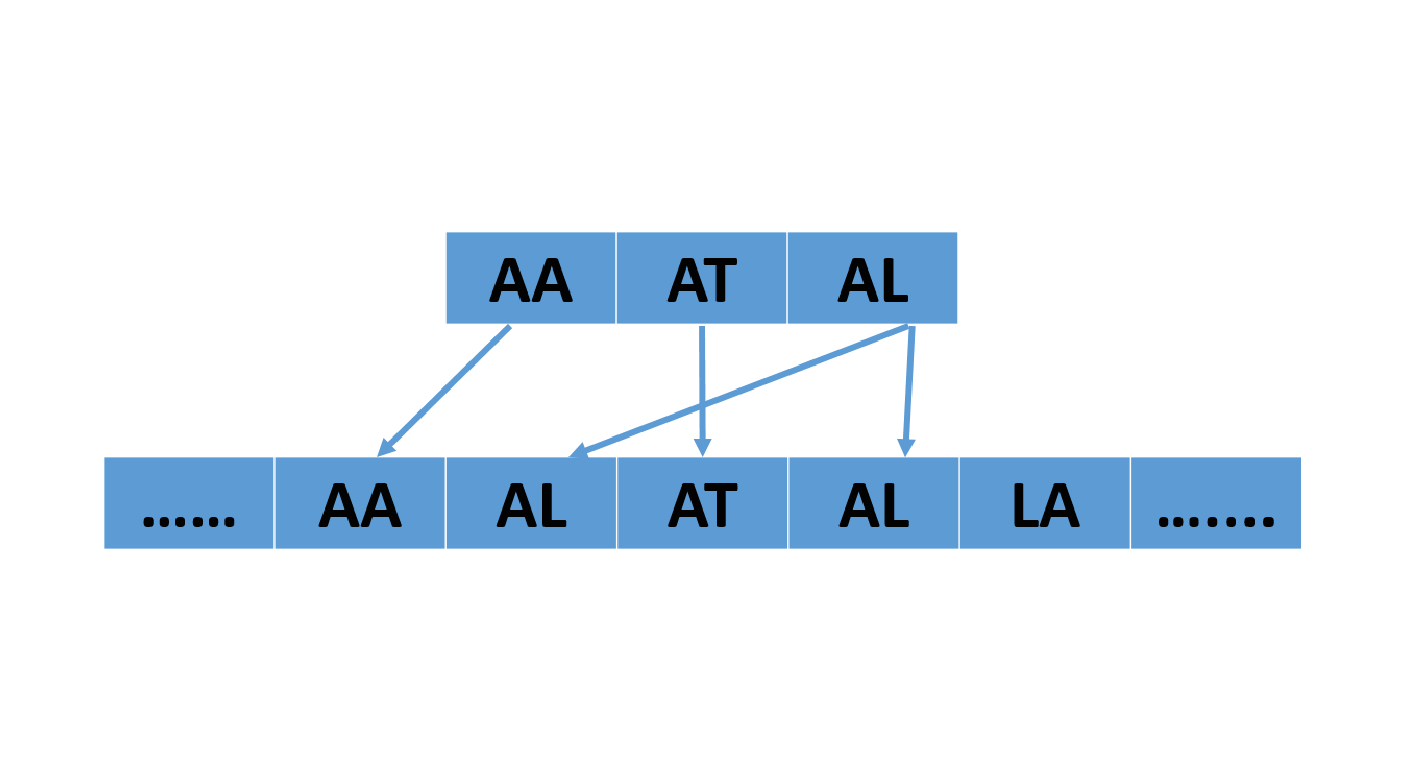
\includegraphics[width=0.7\textwidth]{Dipeptidenew.eps}
 %\caption*{\scriptsize Source:\url{https://www.kyowa.eu/products/new-products/dipeptides.html}}
 \caption{Dipeptide Composition}
\end{figure}

\subsection{Tripeptide Composition}
We have also considered tripeptide composition which is the normalized frequency of tripeptides. The total number of tripeptides are 8000. Here monomer composition is represented by $f_3$.

\begin{figure}[H]
\centering
 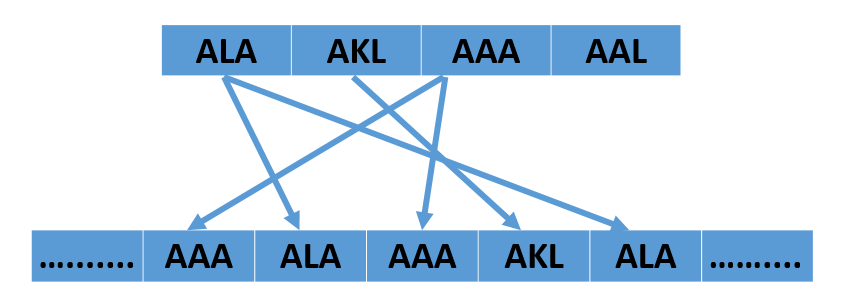
\includegraphics[width=0.7\textwidth]{tripeptide.PNG}
 %\caption*{\scriptsize Source:\url{https://www.kyowa.eu/products/new-products/dipeptides.html}}
 \caption{Tripeptide Composition}
\end{figure}

\subsection{1-gapped Di-mono Composition}
We have also considered the normalized frequency of tripeptides with a single gap in them. The particular patterns are in the form of $XX\_X$. The number of features are 8000.

\begin{figure}[H]
\centering
 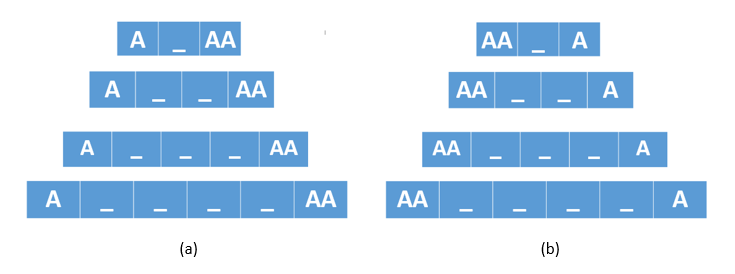
\includegraphics[width=0.7\textwidth]{comGap.PNG}
 %\caption*{\scriptsize Source:\url{https://www.kyowa.eu/products/new-products/dipeptides.html}}
 \caption{(a) 1-gapped Mono-Di Composition and (b) 1-gapped Di-mono Composition}
\end{figure}

\subsection{1-gapped Mono-Di Composition}
Similarly we have also considered normalized frequency of tripeptides with a single gap in them in the form of $X\_XX$. The number of features are 8000.

\subsection{Feature Collection Summary}
We have divided the generated features into three non-overlapping groups. Summary of the features and subspacing are given in Table~\ref{tab:features}.

\begin{table}[h]
    \centering
    \begin{tabular}{c| c| c| r}
        Feature Subspace & Features & Type & Number of features \\
        \hline
        $G_1$ & $f_1$ & Monomer Composition & 20\\
        & $f_2$& Dipeptide Composition & 400\\
        & $f_3$& Tripeptide Composition & 8000\\
        \hline 
        $G_2$ & $f_4$ & 1-gapped Di-mono Composition & 8000\\
        \hline 
        $G_3$ & $f_5$ & 1-gapped Mono-Di Composition & 8000\\
    \end{tabular}
    \caption{Summary of features and feature subspacing.    \label{tab:features}}

\end{table}

\section{Classification Algorithm}
We have used a feature subspacing based ensemble classification algorithm as a classifier in this work. Fig.~\ref{fig:en} shows a block diagram for the classifier used. After the feature extraction phase, the total number of feature are divided into three groups as shown in the figure and also in Table~\ref{tab:features}. Each of these feature vectors are then zipped with the peptide labels to train individual classifiers. Since there are three parts, we will need three different classifiers for training.  
\begin{figure}[h]
    \centering
    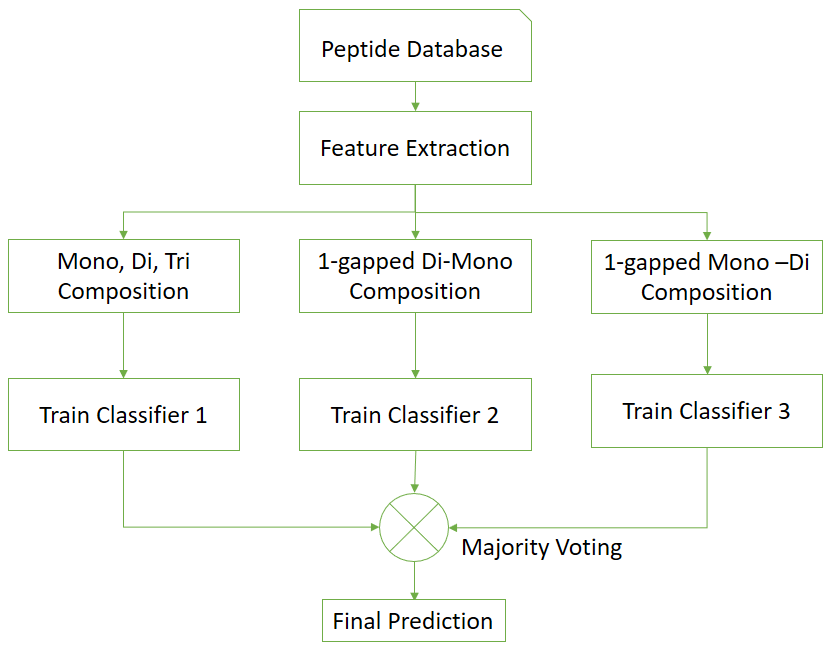
\includegraphics[width=0.8\textwidth]{ensemble}
    \caption{Block diagram of the feature subspacing ensemble classifier.     \label{fig:en}}
\end{figure}

Note that three single classifiers used to train three subspaces of the feature space are not required to be of the same type. After the training each will learn their own model and predictions from each of these single classifiers will be aggregated using a simple majority voting for the final prediction. In the testing phase three models are to be saved in order to be used along with the voting scheme. Note that, we have not utilized any weighted voting here. Also the choice of dividing the feature space into three parts was also done arbitrarily. Weighted schemes, overlapped feature subspacing and number of subspaces could be left for future exploration. 

\section{Used Algorithm}
We used K nearest neighbor\cite{Anderson07}, naive bayesian\cite{Anderson08}\cite{Anderson09}, support vector machine\cite{Anderson10}, decision tree\cite{safavian1991survey} and logistic regression\cite{hosmer2013applied} for predicting the result.

\section{Parameter of Using Algorithms}
The table shows the parameter of algorithms.
\begin{table}[htbp]
\caption[Parameter of Algorithm]{Parameter of Algorithm }
\centering
\footnotesize
\resizebox{\textwidth}{!}{\begin{tabular}{|c| >{\centering\arraybackslash}p{3.5cm} |c|} \hline
\bf Classifier & \bf Parameters & \bf Types \\\hline
K-Nearest Neighbor & Number of Neighbors, Training set, test instances and defaults & -  \\\hline
Naïve Bayes & Training set, test instances and defaults & Bernoulli \\\hline
Support Vector Machine & Training set, test instances and defaults & Support Vector Classifier \\\hline
Decision Tree & Training set, test instances and defaults & - \\\hline
Logistic Regression & Training set, test instances and defaults & -  \\\hline

\end{tabular}}
%\label{training_testing_examples_KDD99}
\end{table}

\section{Performance Evaluation}
In the literature of supervised learning methods for any prediction task, it is shown that selection of performance evaluation methods in very important \cite{chou2011some}. For the sake of comparison, we have used the standard set of metrics and evaluation methods for the performance evaluation of our method as well. We have used 10-fold cross validation technique for the sampling on the train set. Here, the train set is divided into 10 folds or parts shuffled randomly and each time, a single fold in used as testing while the rest of the dataset is used for training. 

We have used eight standard metrics for as performance measure: Accuracy (Acc), Sensitivity (Sn), Specificity (Spc), Precision, Recall, F1-Score, Matthew's Correlation Coefficient (MCC) and area under Receiver Operating Characteristic curve (auROC). For any binary classification task, we assume $TP$ be the number of true positives or number of correctly predicted positive instances and $TN$ be the number of true negatives or number of correctly predicted negative instances. Let FP and FN denote number of false positive and false negatives. They are respectively negative instances incorrectly predicted as positive and  positive instances incorrectly predicted as negative. Now the metrics are defined as in below:    

\small{
\[ Acc = \frac{TP + TN}{TP + FP + FN + TN} \times 100\% \]
\[ Sn = \frac{TP}{TP + FN} \times 100\% \]
\[ Spc = \frac{TN}{TN + FP} \times 100\% \]
\[ Precision = \frac{TP}{TP + FP} \]
\[ Recall = \frac{TP}{TP + FN}\]
\[ F1-Score = \frac{2 \times precision \times recall}{precision + recall}\]
\scriptsize{
\[ MCC = \frac{(TP \times TN) - (FN \times FP)}{\sqrt{(TP+FN) \times (TN+FP) \times (TP+FP) \times (TN+FN)}} \]
}}

We have also considered auROC or area under Receiver Operating Characteristic (ROC) curve. ROC curve is the plot of TPR against FPR for different thresholds from a probabilistic classifier. Here note that each of this measures have the values in the range [0,1] except MCC. Here 0 means a worst classifier and 1 means a perfect classifier. In the case of MCC the values are in the range of [-1,+1]. 

\section{Summary}

In this chapter we have discussed about our collected features, our used algorithms.


